\documentclass[12pt, dvipsnames, svgnames, x11names,]{article}

\usepackage{xcolor}
% URLs and hyperlinks ---------------------------------------
\usepackage{hyperref}
\hypersetup{
	colorlinks=true,
	linkcolor=NavyBlue,
	filecolor=magenta,      
	urlcolor=blue,
}
\usepackage{xurl}
%---------------------------------------------------
\usepackage[inline]{enumitem}
\usepackage{graphicx}
\usepackage{multirow}
\usepackage{float}
\renewcommand{\arraystretch}{1.40}

% adjust a verrrrry big table -------------------------------
\usepackage{adjustbox}
% -----------------------------------------------------------

\usepackage{array}
% center the p columns and m --------------------------------------------------------------
\newcolumntype{P}[1]{>{\centering\arraybackslash}p{#1}}
\newcolumntype{M}[1]{>{\centering\arraybackslash}m{#1}}
% -------------------------------------------------------------------------------------------------------------

% price
\usepackage{marvosym}
% ----------

\usepackage{xepersian}
\settextfont{Arial}
\setdigitfont{Arial}

\begin{document}
	\begin{titlepage}
		\centering
		
		\centering
		
\includegraphics[width=3.2cm, height=3.2cm]{images/image001}\par
		\vspace{5mm}
		{\large دانشگاه اصفهان}\par
		\vspace{5mm}
		{\large دانشکده مهندسی کامپیوتر}\par
		
		\vspace{1cm}
		{\Large {\textbf{آموزش مدل \lr{MLP} بر روی داده‌های \lr{MNIST}}}\par}
		\vspace{15mm}
		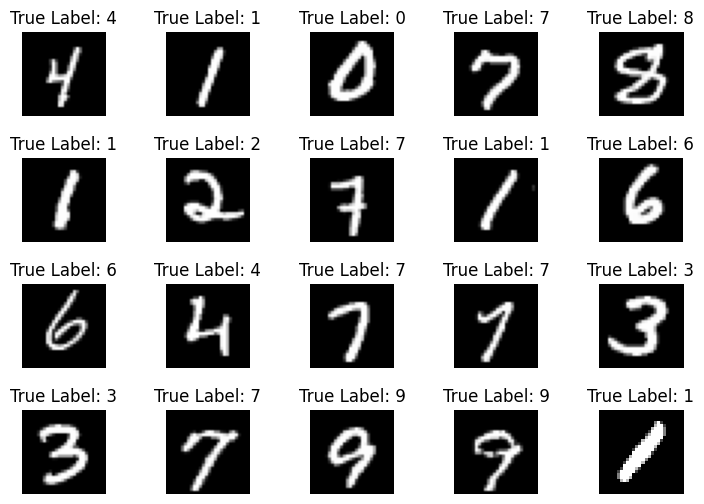
\includegraphics[width=9cm]{images/00.png} \par
		\vfill \par	\vfill
		\vspace{16mm}
		{\normalsize	سیدمحمدحسین هاشمی  4022363143 \par}
		\vspace{1cm}
		{\large خرداد ۱۴۰3\par}
	\end{titlepage}
	
	\clearpage
	\begin{center}
		
\includegraphics[width=10cm]{images/image002}
	\end{center}  
	\thispagestyle{plain}\mbox{} 
	\clearpage

	\tableofcontents
	\newpage
	
	\begin{abstract}
		در دنیای هوش مصنوعی و یادگیری ماشین، شبکه‌های عصبی مصنوعی (\lr{ANNs}) نقش بسیار مهمی در پردازش و تحلیل داده‌ها ایفا می‌کنند. یکی از معروف‌ترین و پرکاربردترین انواع این شبکه‌ها، شبکه عصبی پرسپترون چندلایه (\lr{MLP}) است. \lr{MLP} یکی از ساده‌ترین انواع شبکه‌های عصبی پیش‌خور\LTRfootnote{feedforward} محسوب می‌شود که شامل یک یا چند لایه مخفی\LTRfootnote{hidden layers} بین لایه ورودی و خروجی است. 
		
		دیتاست \lr{MNIST}\LTRfootnote{Modified National Institute of Standards and Technology} یکی از این دیتاست‌هاست که به عنوان معیار استاندارد در بسیاری از پروژه‌های یادگیری ماشین و بینایی ماشین استفاده می‌شود. دیتاست \lr{MNIST} شامل 60000 تصویر آموزشی و 10000 تصویر تست از ارقام دست‌نویس 0 تا 9 است. هر تصویر در این دیتاها به صورت یک ماتریس 28x28 پیکسل بوده و هر پیکسل مقداری بین 0 تا 255 را نشان می‌دهد که شدت رنگ خاکستری را نمایان می‌سازد.
		
		آموزش یک \lr{MLP} بر روی دیتاست \lr{MNIST} به ما کمک می‌کند تا نحوه عملکرد این نوع شبکه‌ها را در تشخیص الگوهای پیچیده‌تر و طبقه‌بندی داده‌ها بهتر بفهمیم. در این فرآیند، مراحل مختلفی مانند پیش‌پردازش داده‌ها، طراحی و ساختاردهی شبکه، آموزش و ارزیابی مدل را باید طی کنیم.
	\end{abstract}
	
	
	\section{تعداد لایه‌های مخفی}
		در انتخاب تعداد لایه‌های مخفی\LTRfootnote{Hidden Layers} برای شبکه عصبی پرسپترون چندلایه (\lr{MLP})، یکی از مهمترین ملاحظات، یافتن توازنی بین دقت آموزش و تست و همچنین پیچیدگی مدل است. نمودار ارائه شده نشان می‌دهد که چگونه تعداد لایه‌های مخفی بر دقت آموزش، دقت تست و تعداد تکرارهای لازم برای رسیدن به همگرایی تاثیر می‌گذارد. در شکل \ref{fig:hidden_layers} به مقایسه تعداد لایه‌ها در عملکرد شبکه پرداخته‌ایم.
		
	\begin{figure}
		\begin{center}
			{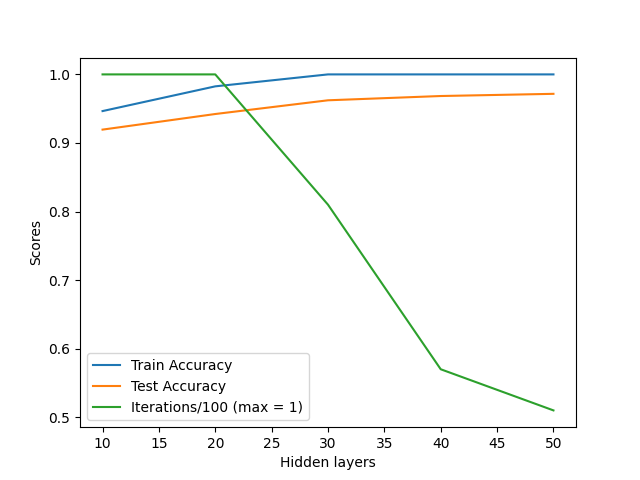
\includegraphics[width=10cm]{images/01.png}}
		\end{center}
		\caption{تعداد لایه‌های مخفی}
		\label{fig:hidden_layers}
	\end{figure}
		
		
		دقت آموزش (\lr{Train Accuracy}): با افزایش تعداد لایه‌های مخفی، دقت آموزش به طور کلی افزایش یافته و در حدود 30 لایه به نقطه اشباع می‌رسد. این نشان می‌دهد که افزودن لایه‌های بیشتر بعد از این نقطه تاثیر قابل توجهی در بهبود دقت آموزش ندارد.
		
		
		دقت تست (\lr{Test Accuracy}): دقت تست نیز روند مشابهی را دنبال می‌کند و با افزایش تعداد لایه‌های مخفی بهبود می‌یابد تا به نقطه‌ای اشباع در حدود 30 لایه برسد. بعد از این نقطه، دقت تست بهبود قابل توجهی نمی‌یابد.
		
		
		تعداد تکرارها (\lr{Iterations}): تعداد تکرارهای لازم برای همگرایی شبکه با افزایش تعداد لایه‌های مخفی کاهش می‌یابد. این نشان می‌دهد که پیچیدگی شبکه بعد از یک نقطه مشخص (حدود 20 لایه) باعث کاهش زمان آموزش می‌شود و شبکه سریع‌تر به همگرایی می‌رسد. هرچند باید به این نکته نیز توجه داشت که تعداد لایه‌های بیشتر باعث می‌شود هرتکرار محاسبات بیشتری نیاز داشته باشد.
		
		
		نتیجه‌گیری:
		با توجه به نمودار، به نظر می‌رسد که تعداد بهینه لایه‌های مخفی برای این شبکه در حدود 30 - 50 لایه است. در این محدوده، دقت آموزش و تست به بیشترین مقدار خود نزدیک شده و تعداد تکرارهای لازم برای همگرایی نیز در حداقل مقدار ممکن است. انتخاب تعداد لایه‌های بیشتر از این مقدار ممکن است منجر به پیچیدگی اضافی و زمان آموزش بیشتر بدون بهبود قابل توجه در دقت مدل شود.
		
		توصیه‌ها:
		انتخاب بهینه تعداد لایه‌ها: بر اساس نمودار، 50 لایه مخفی می‌تواند انتخاب مناسبی برای مدل \lr{MLP} باشد.
		
		
		اجتناب از بیش‌برازش (\lr{Overfitting}): افزودن لایه‌های بیشتر می‌تواند به بیش‌برازش منجر شود که در آن مدل به خوبی بر روی داده‌های آموزش عمل می‌کند ولی دقت آن بر روی داده‌های تست کاهش می‌یابد.
		کارایی مدل: با توجه به پیچیدگی محاسباتی و زمان آموزش، انتخاب تعداد لایه‌های بهینه می‌تواند به افزایش کارایی و کاهش هزینه‌های محاسباتی کمک کند.
		
		
		به این ترتیب، با توجه به تحلیل نمودار و بررسی دقت آموزش و تست و همچنین تعداد تکرارهای لازم برای همگرایی، انتخاب تعداد لایه‌های مخفی در حدود 50 لایه به عنوان یک انتخاب بهینه پیشنهاد می‌شود.
	
	
	\section{تعداد نورون‌های هرلایه}
		
		انتخاب تعداد نورون‌های هر لایه در شبکه عصبی پرسپترون چندلایه (MLP) یکی از مسائل مهم در طراحی شبکه است. هدف از این انتخاب، دستیابی به بالاترین دقت در آموزش و تست و همچنین کمترین تعداد تکرارهای لازم برای همگرایی است. نمودار ارائه شده، تاثیر تعداد نورون‌ها در هر لایه را بر دقت آموزش\LTRfootnote{Train Accuracy}، دقت تست\LTRfootnote{Test Accuracy}، و تعداد تکرارهای لازم برای همگرایی\LTRfootnote{Iterations} نشان می‌دهد. در شکل \ref{fig:hidden_layer_size} به مقایسه تعداد لایه‌ها در عملکرد شبکه پرداخته‌ایم.
				
		\begin{figure}
			\begin{center}
				{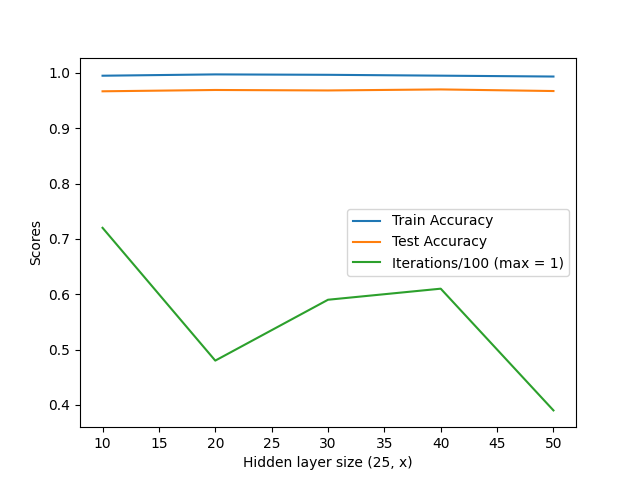
\includegraphics[width=10cm]{images/02.png}}
			\end{center}
			\caption{تعداد نورون‌ها در لایه‌های مخفی}
			\label{fig:hidden_layer_size}
		\end{figure}
		
		تحلیل نمودار:
		دقت آموزش (\lr{Train Accuracy}): با توجه به نمودار، دقت آموزش تقریباً ثابت و نزدیک به 1 (100 \%) باقی می‌ماند که نشان می‌دهد مدل به خوبی قادر به یادگیری داده‌های آموزش است.
		
		
		دقت تست (\lr{Test Accuracy}): دقت تست نیز ثابت و نزدیک به 1 (100 \%) باقی مانده و با تغییر تعداد نورون‌ها تفاوت چندانی ندارد، که نشان‌دهنده توانایی خوب مدل در تعمیم به داده‌های جدید است.
		
		
		تعداد تکرارها (\lr{Iterations}): تعداد تکرارهای لازم برای همگرایی شبکه با تغییر تعداد نورون‌ها در هر لایه تغییر می‌کند. کمترین تعداد تکرارها در حدود 50 نورون در هر لایه به دست می‌آید، در حالی که با افزایش یا کاهش تعداد نورون‌ها، تعداد تکرارها ابتدا افزایش و سپس کاهش می‌یابد.
		
		
		نتیجه‌گیری:
		با توجه به نمودار، به نظر می‌رسد که تعداد بهینه نورون‌ها در هر لایه حدود 20 تا 30 نورون است. در این محدوده، دقت آموزش و تست به حداکثر مقدار خود نزدیک بوده و تعداد تکرارهای لازم برای همگرایی نیز در کمترین مقدار خود است.
		
		
		توصیه‌ها:
		انتخاب بهینه تعداد نورون‌ها: بر اساس نمودار، تعداد نورون‌های هر لایه در محدوده 20 تا 30 می‌تواند انتخاب مناسبی برای مدل \lr{MLP} باشد.
		
		
		اجتناب از پیچیدگی اضافی: افزایش یا کاهش شدید تعداد نورون‌ها می‌تواند منجر به افزایش پیچیدگی محاسباتی و زمان آموزش بدون بهبود قابل توجه در دقت مدل شود.
		
		
		کارایی مدل: با انتخاب تعداد بهینه نورون‌ها، کارایی مدل افزایش یافته و هزینه‌های محاسباتی کاهش می‌یابد.
		
		جمع‌بندی:
		با توجه به تحلیل نمودار و بررسی دقت آموزش و تست و همچنین تعداد تکرارهای لازم برای همگرایی، انتخاب تعداد نورون‌های هر لایه در محدوده 20 تا 30 به عنوان یک انتخاب بهینه پیشنهاد می‌شود. این انتخاب باعث می‌شود مدل با دقت بالا و زمان آموزش کمتر به همگرایی برسد و عملکرد مناسبی در طبقه‌بندی داده‌ها داشته باشد.
		
		
		به این ترتیب، با توجه به دقت آموزش و تست بالا و تعداد تکرارهای کم، می‌توان گفت که انتخاب تعداد نورون‌های هر لایه در محدوده 20 تا 30 نورون بهینه است و می‌تواند بهترین نتیجه را در آموزش مدل \lr{MLP} بر روی دیتابیس \lr{MNIST} به همراه داشته باشد.
	
	
	\section{توابع بهینه سازی}
		در کتابخانه \lr{scikit-learn}\LTRfootnote{sklearn} در \lr{Python}، توابع بهینه سازی که برای آموزش مدل های \lr{MLP}\LTRfootnote{Multi-Layer Perceptron} استفاده می‌شوند عبارتند از:
		
		\subsection{تابع بهینه‌سازی \lr{SGD}}
		
			\begin{itemize}
				
				\item \lr{SGD}\LTRfootnote{Stochastic Gradient Descent} یک الگوریتم بهینه سازی اول مرتبه است که برای آموزش مدل های ماشین یادگیری استفاده می شود.
				
				\item در این روش، به جای استفاده از گرادیان کل داده ها، از نمونه های تصادفی از داده ها برای محاسبه گرادیان استفاده می شود.
				
				\item این روش محاسبات را ساده تر و کارآمدتر می کند و برای مقیاس پذیری مناسب است.
				
				\item \lr{SGD} معمولاً برای مدل های بزرگ و داده های با حجم زیاد مناسب است.
				
				
			\end{itemize}
			
			
		\subsection{تابع بهینه‌سازی \lr{L-BFGS}}
		
			\begin{itemize}
				
				\item \lr{L-BFGS}\LTRfootnote{Limited-memory Broyden-Fletcher-Goldfarb-Shanno} یک الگوریتم بهینه سازی مرتبه دوم است که از تقریب ماتریس هسین استفاده می کند.
				
				\item این روش به جای محاسبه مستقیم ماتریس هسین، از یک ساختار داده ای کم حافظه برای نگهداری اطلاعات مربوط به ماتریس هسین استفاده می کند.
				
				\item \lr{L-BFGS} همگرایی سریع تری نسبت به \lr{SGD} دارد و برای مسائل با فضای پارامتری کوچک تر مناسب است.
				
				\item این روش محاسبات پیچیده تری نسبت به \lr{SGD} دارد، اما همچنان در مقایسه با روش های مرتبه دوم سنتی کارآمد است.
				
			\end{itemize}
		
		
		\subsection{تابع بهینه‌سازی \lr{Adam}}
			
			\begin{itemize}
				
				\item \lr{Adam}\LTRfootnote{Adaptive Moment Estimation} یک الگوریتم بهینه سازی است که از محاسبات گرادیان تطبیقی برای آموزش مدل های ماشین یادگیری استفاده می کند.
				
				\item در این روش، به جای تنظیم نرخ یادگیری به صورت ثابت، نرخ یادگیری به صورت تطبیقی برای هر پارامتر بروز رسانی می شود.
				
				\item \lr{Adam} از میانگین متحرک گرادیان و مربع گرادیان برای تنظیم نرخ یادگیری استفاده می کند.
				
				\item \lr{Adam} در مقایسه با روش های بهینه سازی سنتی مانند \lr{SGD}، همگرایی سریع تری دارد و برای مسائل پیچیده مناسب است.
				
			\end{itemize}
		
		\subsection{مقایسه سه روش}
			
			نمودار مقایسه این سه تابع بهینه سازی را در تصاویر \ref{fig:func:train}، \ref{fig:func:test} و \ref{fig:func:iteration} و نتیجه مقایسه این سه روش را در \ref{table:func} مشاهده می‌کنید.
			
			\begin{figure}
				\begin{center}
					{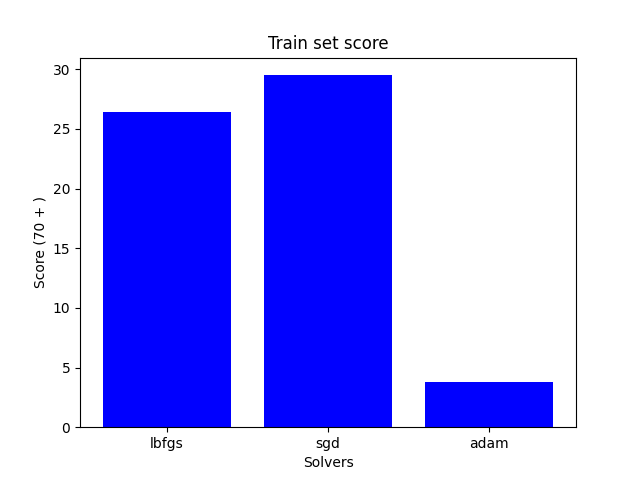
\includegraphics[width=10cm]{images/03.png}}
				\end{center}
				\caption{مقایسه دقت آموزش در توابع}
				\label{fig:func:train}
			\end{figure}
			
			\begin{figure}
				\begin{center}
					{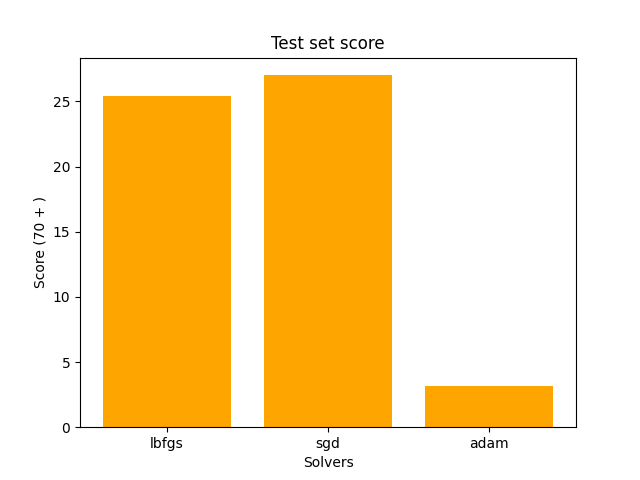
\includegraphics[width=10cm]{images/04.png}}
				\end{center}
				\caption{مقایسه دقت تست در توابع}
				\label{fig:func:test}
			\end{figure}
			
			\begin{figure}
				\begin{center}
					{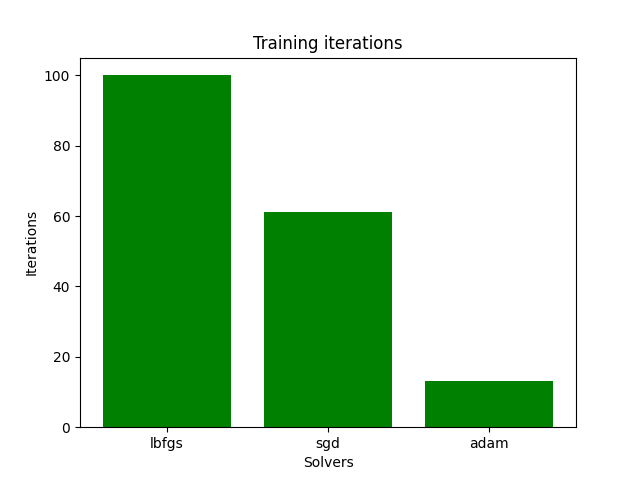
\includegraphics[width=10cm]{images/05.png}}
				\end{center}
				\caption{مقایسه تعداد تکرار در توابع}
				\label{fig:func:iteration}
			\end{figure}
			
			
			\begin{table}[H]
				\caption{مقایسه توابع بهینه سازی}
				\label{table:func}
				\begin{center}
					\begin{adjustbox}{width=8cm}
						\begin{tabular}{|c|c|c|c|}
							\hline
							دقت آموزش
							&
							دقت تست
							&
							تعداد تکرار
							&
							تابع بهینه سازی
							\\ 
							\hline
							بالا
							&
							بالا
							&
							بالا
							&
							\lr{L-BFGS}
							\\
							\hline
							بالا
							&
							بالا
							&
							پایین
							&
							\lr{SGD}
							\\
							\hline
							پایین
							&
							پایین
							&
							پایین
							&
							\lr{Adam}
							\\
							\hline
						\end{tabular}
					\end{adjustbox}
				\end{center}
			\end{table}
	
		نتیجه گیری: طبق نتایج دریافت شده واضح است که استفاده از تابع بهینه‌سازی \lr{SGD} علاوه بر دقت بالا در آموزش و تست به تعداد تکرار کمتری نیز برای آموزش نیاز دارد.
	
	
	\section{توابع فعال سازی}
	
		توابع فعال‌سازی در شبکه‌های عصبی یکی از اجزای کلیدی هستند که نقش مهمی در عملکرد و یادگیری مدل‌ها دارند. در کتابخانه \lr{Scikit-Learn} نیز توابع فعال‌سازی مختلفی برای استفاده در مدل‌های عصبی وجود دارند. در ادامه، به توضیح مختصری از تعدادی از توابع فعال‌سازی موجود در \lr{Scikit-Learn} می‌پردازیم:
	
		
		\subsection{\lr{Identity}}
		
			\begin{itemize}
				
				\item این تابع هیچ تغییری در ورودی ایجاد نمی‌کند و خروجی همان ورودی است.
				
				\item فرمول آن به صورت زیر است:
				\begin{center}
					\lr{$
						f(x) = x
						$}
				\end{center}
				
			\end{itemize}
			
		\subsection{\lr{ReLU (Rectified Linear Unit)}}
				
			\begin{itemize}
				
				\item این تابع برای حذف خطی‌تر کردن خروجی نورون‌ها استفاده می‌شود.
				
				
				\item فرمول آن به صورت زیر است:
				
				\begin{center}
					\lr{$
						f(x) = \max(0, x)
						$}
				\end{center}
				
			\end{itemize}
		
		\subsection{\lr{Logistic (Sigmoid)}}
		
			\begin{itemize}
				
				\item این تابع برای مسائل طبقه‌بندی دو کلاسه استفاده می‌شود.
				
				\item فرمول آن به صورت زیر است:
				
				\begin{center}
					\lr{$
						f(x) = \frac{1}{1 + e^{-x}}
						$}
				\end{center}
				
				
			\end{itemize}
		
		\subsection{\lr{Tanh (Hyperbolic Tangent)}}
		
			\begin{itemize}
				
				\item این تابع مقادیر خروجی را در بازه \lr{[-1, 1]} قرار می‌دهد.
				
				\item فرمول آن به صورت زیر است:

				\begin{center}
					\lr{$
						f(x) = \frac{{1 - e^{-2x}}}{{1 + e^{-2x}}}
						$}
				\end{center}
				
			\end{itemize}
			
		
		مقایسه: مدل را با استفاده از هر سه تابع آموزش داده و نتایج را باهم مقایسه می‌کنیم. نمودار های \ref{fig:atcivation:train}، \ref{fig:atcivation:test} و \ref{fig:atcivation:iteration} نمودار مقایسه توابع فعال سازی و جدول \ref{table:atcivation} نتیجه مقایسه را نشان می‌دهند.
			
			
		\begin{figure}
			\begin{center}
				{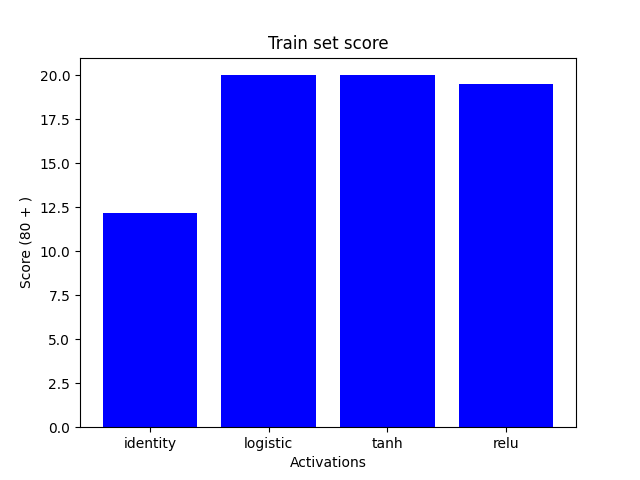
\includegraphics[width=10cm]{images/06.png}}
			\end{center}
			\caption{مقایسه دقت آموزش در توابع}
			\label{fig:atcivation:train}
		\end{figure}
		
		\begin{figure}
			\begin{center}
				{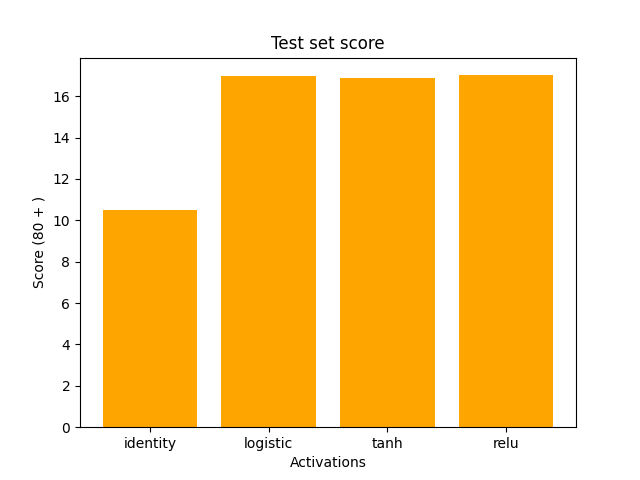
\includegraphics[width=10cm]{images/07.png}}
			\end{center}
			\caption{مقایسه دقت تست در توابع}
			\label{fig:atcivation:test}
		\end{figure}
		
		\begin{figure}
			\begin{center}
				{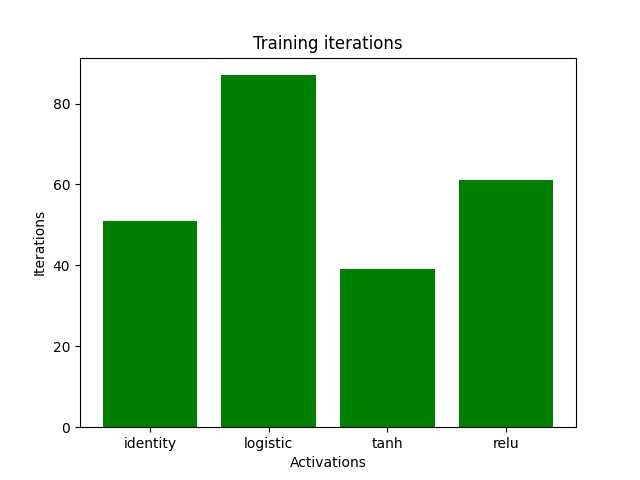
\includegraphics[width=10cm]{images/08.png}}
			\end{center}
			\caption{مقایسه تعداد تکرار در توابع}
			\label{fig:atcivation:iteration}
		\end{figure}
		
		
		\begin{table}[H]
			\caption{مقایسه توابع بهینه سازی}
			\label{table:atcivation}
			\begin{center}
				\begin{adjustbox}{width=8cm}
					\begin{tabular}{|c|c|c|c|}
						\hline
						دقت آموزش
						&
						دقت تست
						&
						تعداد تکرار
						&
						تابع فعال سازی
						\\ 
						\hline
						متوسط
						&
						متوسط
						&
						متوسط
						&
						\lr{identity}
						\\
						\hline
						بالا
						&
						بالا
						&
						بالا
						&
						\lr{logistic}
						\\
						\hline
						بالا
						&
						بالا
						&
						پایین
						&
						\lr{tanh}
						\\
						\hline
						بالا
						&
						بالا
						&
						متوسط
						&
						\lr{relu}
						\\
						\hline
					\end{tabular}
				\end{adjustbox}
			\end{center}
		\end{table}	
		
		
		نتیجه‌گیری: استفاده از \lr{tanh} به نسبت سایر توابع فعال سازی، علاوه بر دقت بالا در آموزش و تست، به تعداد تکرار کمتری برای آموزش نیاز دارد.
		
		
		\section{نرخ یادگیری}
		
			نرخ یادگیری\LTRfootnote{Learning Rate} در شبکه‌های عصبی یک پارامتر بسیار مهم است. این مقدار عددی که در آموزش مدل با روش کاهش شیب\LTRfootnote{gradient descent} استفاده می‌شود، تعیین می‌کند که مدل چقدر سریع یاد می‌گیرد. در هر گام، الگوریتم کاهش شیب مقدار نرخ یادگیری را در گرادیان‌ها یا شیب‌ها ضرب می‌کند. حاصل ضرب این‌ها گام شیب نامیده می‌شود.
			
			نرخ یادگیری یک ابرپارامتر\LTRfootnote{hyperparameter} کلیدی است. انتخاب مناسب نرخ یادگیری می‌تواند تأثیر زیادی بر عملکرد مدل داشته باشد. اگر نرخ یادگیری بزرگ باشد، ممکن است مدل به سرعت همگرا شود، اما به مشکلاتی مانند شلوغی یا نوسان‌های ناپایدار برخورد کند. اگر نرخ یادگیری کوچک باشد، مدل به طور کامل همگرا نشود یا به سرعت در مینیمم محلی گیر کند.
			
			برای تعیین نرخ یادگیری مناسب، معمولاً از روش‌های آزمون و خطا، تجربی، و تنظیم دستی استفاده می‌شود. همچنین الگوریتم‌های پیشرفته‌تری نیز برای تعیین نرخ یادگیری به کار می‌روند.
			
			در کل، انتخاب نرخ یادگیری به تجربه و آزمون‌های مکرر بر مدل‌ها برمی‌گردد تا بهترین مقدار برای مسئله‌ی خاص مشخص شود.
			
			در اینجا برای دریافت نرخ یادگیری نموداری مقایسه ای برای مقادیر مختلف را محاسبه کرده‌ایم که این نمودار را در شکل \ref{fig:learning} مشاهده می‌کنید.
			
			نتیجه‌گیری: طبق نمودار پس از نرخ یادگیری \lr{0.55} دقت مدل در آموزش و تست بالای 90\% شده ولی تعداد تکرار بسیار بالاست ولی در مقدار \lr{0.11} علاوه‌بر دقت بالا در آموزش و تست،‌ تکرار کمتری برای آموزش نیاز دارد که در نتیجه برای نرخ یادگیری از مقدار \lr{0.1} تا \lr{0.2} استفاده می‌کنیم.
			
	
		\begin{figure}
			\begin{center}
				{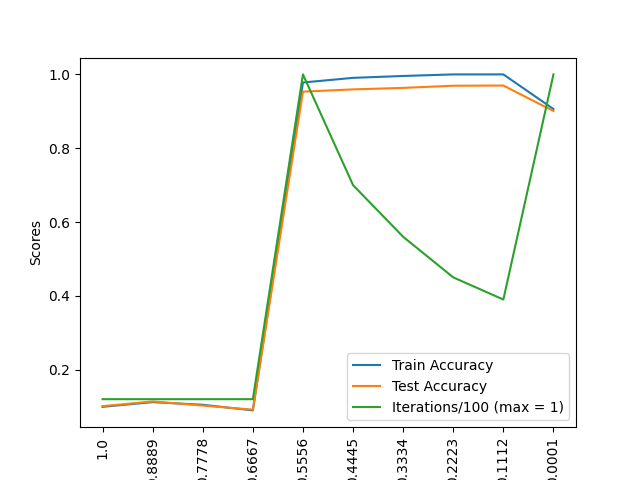
\includegraphics[width=10cm]{images/09.png}}
			\end{center}
			\caption{تاثیر نرخ یادگیری در مدل}
			\label{fig:learning}
		\end{figure}
		
		
	\section{اوورفیتینگ و آندرفیتینگ}
		آندرفیتینگ\LTRfootnote{Underfitting}:
		وقتی مدل خیلی ساده‌ای است و نمی‌تواند الگوهای مهم در داده‌ها را یاد بگیرد، آن را بازتولید کند و یا پیش‌بینی دقیقی انجام دهد، ما آن را آندرفیتینگ می‌نامیم. به عبارت دیگر، مدل آندرفیت شده است و از توانایی کلیه الگوهای موجود در داده‌ها به درستی استفاده نمی‌کند.
		
		اوورفیتینگ\LTRfootnote{Overfitting}:
		وقتی مدل خیلی خود را به داده‌های آموزش برازش می‌کند و الگوهای موجود در داده‌های آموزش را به اندازه‌ی کافی یاد می‌گیرد، اما نتوانسته الگوهای کلی را درک کند و به‌طور کلی بر روی داده‌های جدید عمل نمی‌کند، ما این پدیده را اوورفیتینگ می‌نامیم. به عبارت دیگر، مدل اوورفیت شده است و به داده‌های آموزش بسیار حساس است و به داده‌های جدید عملکرد بدی دارد.
		
		آندرفیتینگ و اوورفیتینگ در شکل \ref{fig:o_under_fitting} مشاهده می‌کنید.

		\begin{figure}
			\begin{center}
				{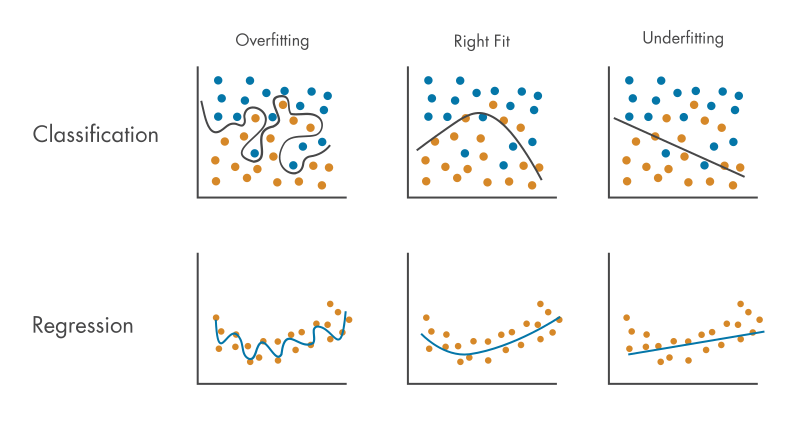
\includegraphics[width=13cm]{images/19.png}}
			\end{center}
			\caption{اوورفیتینگ و آندرفیتینگ}
			\label{fig:o_under_fitting}
		\end{figure}
		
		
	\section{شرایط توقف}
	
		در مدل \lr{MLP} در کتابخانه \lr{scikit-learn}، شرایط توقف مربوط به چندین پارامتر مختلف می‌تواند تعیین شود:
		
		\begin{itemize}
			
			\item \lr{max\_iter}:
			این پارامتر تعیین می‌کند که آموزش مدل تا چند ایپوک ادامه یابد. اگر تعداد ایپوک‌های آموزش به \lr{max\_iter} برسد و مدل هنوز هم به شرایط توقف نرسیده باشد، آموزش متوقف می‌شود.
			
			
			\item \lr{tol}:
			این پارامتر مقدار تعیین‌کننده‌ای است که در صورتی که تغییرات وزن‌های مدل در طول آموزش به آن‌ها کمتر از مقدار مشخص شده باشد، آموزش متوقف می‌شود.
			
			
			\item \lr{early\_stopping}:
			این پارامتر مشخص می‌کند که آیا از شرایط توقف زودهنگام استفاده شود یا خیر. اگر مقدار آن \lr{True} باشد، مدل در صورتی که بهترین عملکرد روی داده‌های اعتبارسنجی بهبود نکند، آموزش متوقف می‌شود.
			
			
			\item \lr{early\_stopping\_patience}:
			این پارامتر تعیین می‌کند که مدل به مدت چند ایپوک بدون بهبود عملکرد روی داده‌های اعتبارسنجی آموزش را ادامه دهد قبل از اینکه تصمیم به توقف بگیرد.
						
			
			\item \lr{n\_iter\_no\_change}:
			این پارامتر تعیین می‌کند که مدل به مدت چند ایپوک بدون بهبود در معیار عملکرد، آموزش را متوقف کند. این پارامتر در صورتی که \lr{early\_stopping} فعال باشد، معنا پیدا می‌کند.

			
			
		\end{itemize}

			با استفاده از ترکیب این پارامترها، می‌توانید شرایط توقف مدل \lr{MLP} را با دقت و کنترل بیشتری مدیریت کنید.
				
		
		
	\section{تاثیر \lr{dropout}}
	
		\lr{Dropout} یکی از روش‌های مهم برای کاهش اوورفیتینگ در شبکه‌های عصبی است. در این روش، به صورت تصادفی برخی از واحدهای (نورون‌ها) در شبکه در هنگام آموزش غیرفعال می‌شوند. به این ترتیب، هر بار که داده از شبکه عبور می‌کند، یک زیرمجموعه مختلف از واحدها غیرفعال می‌شوند و شبکه با اینکه به داده‌های آموزشی تطبیق می‌یابد، از یادگیری وابسته به ویژگی‌های خاص داده‌ها جلوگیری می‌کند.
		
		تاثیر \lr{Dropout} در شبکه‌های عصبی به‌طور خلاصه به شرح زیر است:
		
		\begin{enumerate}
			
			\item کاهش اوورفیتینگ:
			\lr{Dropout} از این اتفاق جلوگیری می‌کند که شبکه به طور زیادی به داده‌های آموزشی برازش شود و الگوهای آموزشی را حفظ کند که ممکن است برای داده‌های تست مناسب نباشد.
			
			\item افزایش عمومیت\LTRfootnote{Generalization}:
			با غیرفعال کردن بخشی از واحدها، شبکه نه تنها به داده‌های آموزشی بلکه به الگوهای کلی و عمومی تری اعمال می‌شود. این باعث می‌شود که شبکه قادر به تعمیم‌پذیری بهتری بر روی داده‌های تست باشد.
			
			\item کاهش وابستگی به ویژگی‌های خاص:
			با غیرفعال کردن بخشی از واحدها، شبکه به یادگیری از ویژگی‌های خاص داده‌ها کمتر وابسته می‌شود و به جای آن الگوهای کلی‌تر و عمومی‌تری را یاد می‌گیرد.
			
		\end{enumerate}
		
		با این وجود، استفاده از \lr{Dropout} نیازمند تنظیمات صحیح است و اعمال \lr{Dropout} به طور نادرست ممکن است عملکرد شبکه را به طرز منفی تحت تأثیر قرار دهد.
		
		در نمودارهای \ref{fig:dropout:test}، \ref{fig:dropout:train} و \ref{fig:dropout:iteration} می‌توانیم تاثیر \lr{Dropout} را مشاهده کنید.
		
	
		\begin{figure}
			\begin{center}
				{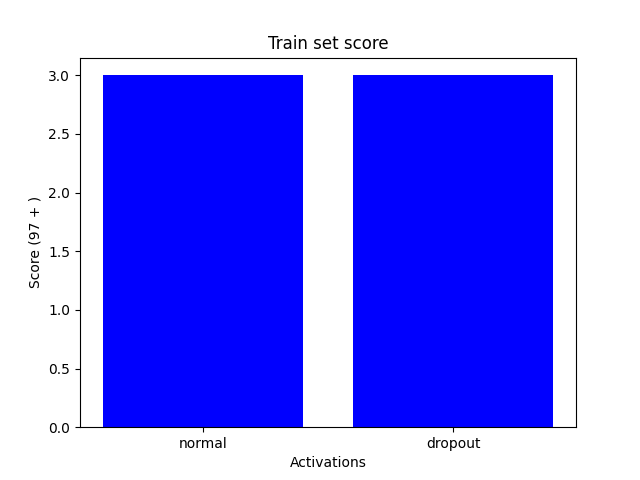
\includegraphics[width=10cm]{images/14.png}}
			\end{center}
			\caption{تاثیر \lr{dropout} در آموزش}
			\label{fig:dropout:train}
		\end{figure}
		
		\begin{figure}
			\begin{center}
				{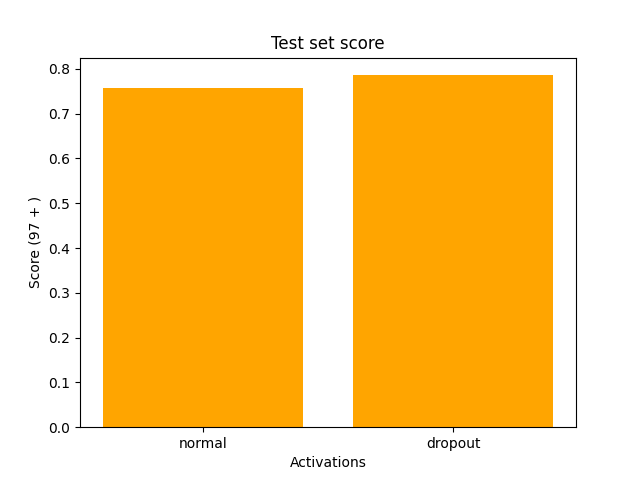
\includegraphics[width=10cm]{images/15.png}}
			\end{center}
			\caption{تاثیر \lr{dropout} در تست}
			\label{fig:dropout:test}
		\end{figure}
		
		\begin{figure}
			\begin{center}
				{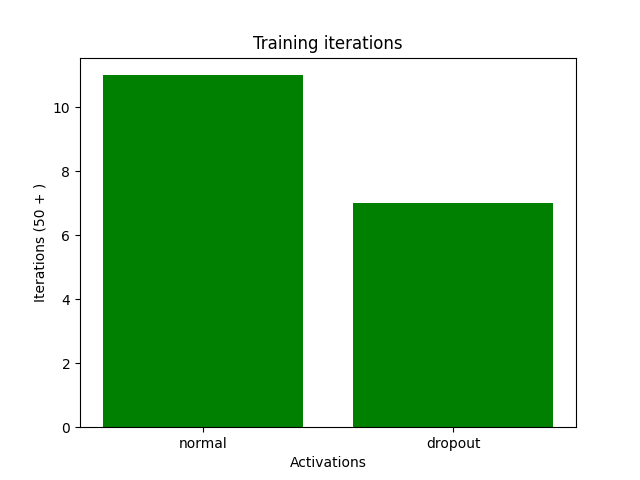
\includegraphics[width=10cm]{images/16.png}}
			\end{center}
			\caption{تاثیر \lr{dropout} در تعداد تکرار}
			\label{fig:dropout:iteration}
		\end{figure}
		
		
	\section{تاثیر \lr{batch\_size}}
	
		انتخاب مناسب \lr{batch\_size} در آموزش شبکه‌های عصبی تأثیر زیادی بر عملکرد و سرعت آموزش دارد. \lr{batch\_size} تعیین می‌کند که در هر مرحله چه تعداد نمونه از داده‌ها برای محاسبه خطا و به‌روزرسانی وزن‌ها استفاده شود. این پارامتر تاثیرات متعددی دارد که به طور خلاصه به شرح زیر است:
		
		\begin{itemize}
			
			\item سرعت آموزش:
			انتخاب \lr{batch\_size} بزرگتر می‌تواند منجر به سرعت بیشتری در آموزش شود. با استفاده از بچ‌های بزرگتر، محاسبات بیشتری همزمان انجام می‌شود که باعث می‌شود فرآیند آموزش سریع‌تر انجام شود.
			
			\item پایداری آموزش:
			با انتخاب \lr{batch\_size} کوچکتر، یعنی استفاده از بچ‌های کوچک‌تر، ممکن است عملکرد شبکه در حین آموزش پایدارتر باشد. این به این معنی است که وزن‌ها به طور متوسط‌تر به‌روزرسانی می‌شوند و در نتیجه آموزش به سمت یک مینیمم محلی نرفته و از مینیمم‌های محلی دیگری نیز گریزان می‌شود.
			
			\item حافظه مصرفی:
			انتخاب \lr{batch\_size} بزرگتر می‌تواند حافظه مصرفی را به طور قابل توجهی کاهش دهد، زیرا تعداد بیشتری از نمونه‌ها در هر مرحله آموزش بارگذاری می‌شوند.
			
			\item دقت آموزش:
			انتخاب مناسب \lr{batch\_size} می‌تواند به دقت آموزش کمک کند. بچ‌های بزرگتر ممکن است باعث شود که شبکه به سرعت به مینیمم محلی برسد و در نتیجه دقت کمتری داشته باشد، در حالی که بچ‌های کوچکتر ممکن است به دقت آموزش کمک کنند.
			
		\end{itemize}
		
		بنابراین، انتخاب \lr{batch\_size} باید با توجه به مسئله و محیط آموزش انجام شود و نیاز به آزمون و خطا برای انتخاب بهترین مقدار دارد.
	
	در شکل \ref{fig:batch_size} تاثیر \lr{batch\_size} را در آموزش،‌ تست و تعداد تکرار مشاهده می‌کنیم.
	
		
		\begin{figure}
			\begin{center}
				{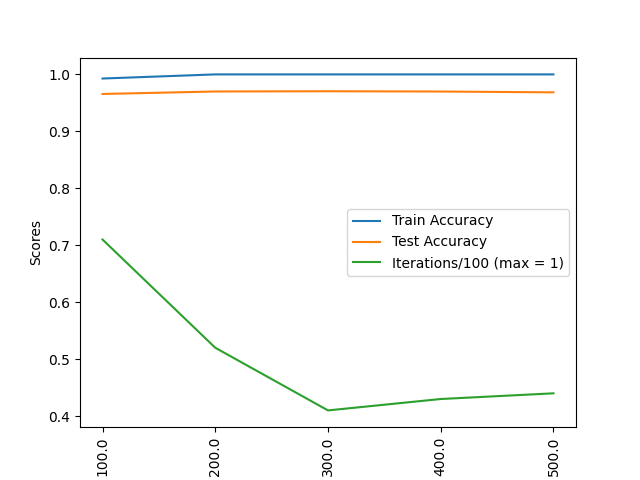
\includegraphics[width=10cm]{images/17.png}}
			\end{center}
			\caption{تاثیر \lr{batch\_size} در مدل}
			\label{fig:batch_size}
		\end{figure}
		
		نتیجه‌گیری: \lr{batch\_size} در مقادیر 250 تا 350 علاوه‌بر افزایش دقت آموزش و تست، تعداد تکرار را نیز کاهش می‌دهد.
		
	\section{مدل نهایی}
	
		در نهایت مدل نهایی با \lr{confusion matrix} شکل \ref{fig:final} به دست می‌آید.
		
		\begin{figure}
			\begin{center}
				{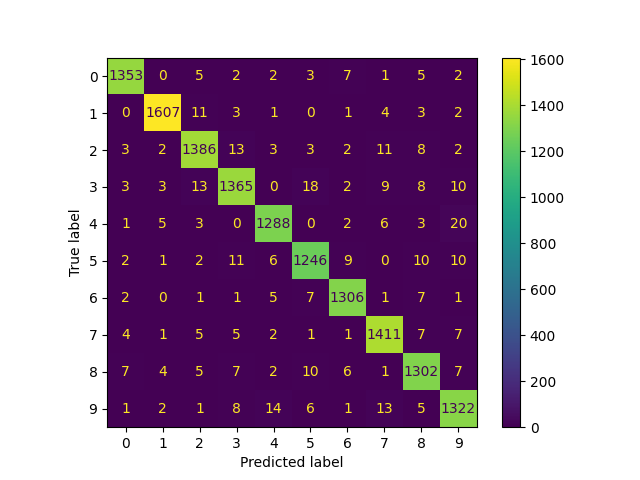
\includegraphics[width=14cm]{images/18.png}}
			\end{center}
			\caption{\lr{confusion matrix} مدل نهایی}
			\label{fig:final}
		\end{figure}
		
\end{document}